%% Specification-Driven Development with OpenSpec
%% Andrii Sukhoi — LKIT 2026
%% Compile: xelatex -shell-escape presentation.tex

\documentclass[aspectratio=169,18pt]{beamer}

%% Theme
\usetheme{Berlin}
\usecolortheme{default}

%% Packages
\usepackage{fontspec}
\usepackage{tikz}
\usetikzlibrary{arrows.meta, positioning, shapes.geometric, fit, backgrounds}
\usepackage{listings}
\usepackage{xcolor}
\usepackage{booktabs}
\usepackage{hyperref}
\usepackage{graphicx}
\usepackage{array}
\usepackage{tabularx}

%% Colors
\definecolor{openblue}{HTML}{2563EB}
\definecolor{opengray}{HTML}{64748B}
\definecolor{opengreen}{HTML}{16A34A}
\definecolor{openred}{HTML}{DC2626}
\definecolor{codbg}{HTML}{1E293B}
\definecolor{codtext}{HTML}{E2E8F0}

\setbeamercolor{frametitle}{bg=openblue, fg=white}
\setbeamercolor{title in head/foot}{bg=openblue, fg=white}
\setbeamercolor{section in head/foot}{bg=openblue!80, fg=white}
\setbeamercolor{normal text}{fg=black}
\setbeamercolor{alerted text}{fg=openblue}

%% Footer
\setbeamertemplate{footline}{%
  \begin{beamercolorbox}[wd=\paperwidth, ht=2.5ex, dp=1.5ex]{footline}%
    \hspace{1em}\scriptsize\color{opengray}Andrii Sukhoi — LKIT 2026%
    \hfill%
    \scriptsize\color{opengray}\insertframenumber\,/\,\inserttotalframenumber\hspace{1em}%
  \end{beamercolorbox}%
}
\setbeamertemplate{navigation symbols}{}

%% Code style
\lstset{
  backgroundcolor=\color{codbg},
  basicstyle=\ttfamily\small\color{codtext},
  breaklines=true,
  frame=none,
  rulecolor=\color{codbg},
  xleftmargin=1em,
  xrightmargin=1em,
}

%% Large fonts globally
\setbeamerfont{frametitle}{size=\large, series=\bfseries}
\setbeamerfont{normal text}{size=\normalsize}

%% Meta
\title{\textbf{Specification-Driven Development\\with OpenSpec}}
\subtitle{\textit{"Agree before you build"}}
\author{Andrii Sukhoi}
\institute{Lubelski Klub IT}
\date{2026}

%% ─────────────────────────────────────────────
\begin{document}

\maketitle

%% ══════════════════════════════════════════════
%% SECTION 1: THE PROBLEM
%% ══════════════════════════════════════════════

%% Slide: About Me
\begin{frame}{About Me}
  \vspace{0.5em}
  \begin{columns}[T]
    \begin{column}{0.6\textwidth}
      \Large
      \textbf{Andrii Sukhoi}\\[1em]
      \normalsize
      \begin{itemize}\setlength\itemsep{0.6em}
        \item Senior Software Engineer
        \item CEO of Dusha Fund
        \item Tennis Instructor
        \item Running 5 AI agents inside myself
      \end{itemize}
      \vspace{1em}
      \texttt{\href{https://github.com/sukhoy94}{\color{openblue}github.com/sukhoy94}}
    \end{column}
    \begin{column}{0.4\textwidth}
      \vspace{1em}
      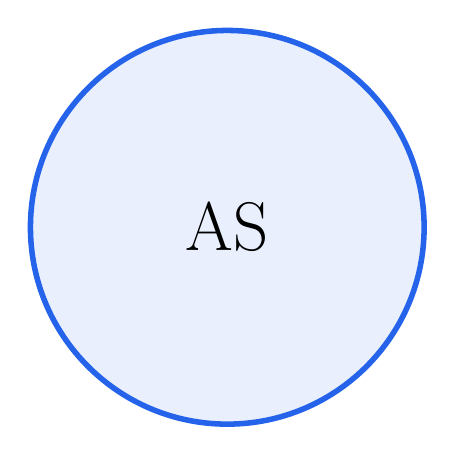
\begin{tikzpicture}
        \node[circle, draw=openblue, line width=2pt, minimum size=5cm,
              fill=openblue!10, font=\Huge] {AS};
      \end{tikzpicture}
    \end{column}
  \end{columns}
\end{frame}

%% Slide: >90%
\begin{frame}{}
  \vspace{2em}
  \begin{center}
    {\fontsize{72}{80}\selectfont\textbf{\color{openblue}>90\%}}\\[0.5em]
    \Large of developers now use AI coding assistants\\[1em]
    \normalsize\color{opengray}— GitHub Developer Survey, 2025
  \end{center}
\end{frame}

%% Slide: But There's a Problem
\begin{frame}{But There's a Problem}
  \vspace{1em}
  \begin{center}
    \Large AI generates code\\[0.5em]
    \textbf{without formal requirements.}\\[1.5em]
    \normalsize
    It works from whatever you typed in chat.\\[0.3em]
    No structure.\quad No memory.\quad No contract.
  \end{center}
\end{frame}

%% Slide: Requirements Live in Chat
\begin{frame}{Requirements Live in Chat}
  \vspace{1em}
  \begin{center}
    \Large\textbf{Chat history is not a specification.}\\[1.5em]
    \normalsize
    Requirements get lost, mutate,\\
    contradict each other across messages.\\[1em]
  \end{center}
  \begin{tikzpicture}[overlay, remember picture]
    \node[opacity=0.15, font=\Huge] at (current page.center) {💬 💬 💬 ?};
  \end{tikzpicture}
\end{frame}

%% Slide: The Result (quote)
\begin{frame}{}
  \vspace{3em}
  \begin{center}
    \Large\textit{"Vague prompts lead to\\[0.3em]
    unpredictable results."}\\[1.5em]
    \normalsize\color{opengray}— OpenSpec Documentation
  \end{center}
\end{frame}

%% ══════════════════════════════════════════════
%% SECTION 2: HOW WE GOT HERE
%% ══════════════════════════════════════════════

\begin{frame}{The Evolution of Software Development}
  \vspace{0.5em}
  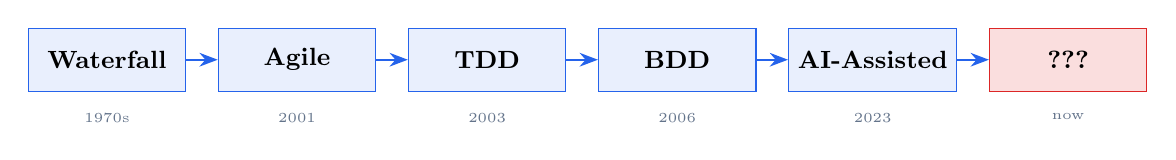
\begin{tikzpicture}[
    node distance=0.4cm,
    box/.style={rectangle, draw=openblue, fill=openblue!10,
                minimum width=2cm, minimum height=0.8cm,
                font=\small\bfseries, text centered},
    arr/.style={-{Stealth}, thick, color=openblue},
    year/.style={font=\tiny\color{opengray}, below=0.15cm}
  ]
    \node[box] (wf) {Waterfall};
    \node[year] at (wf.south) {1970s};

    \node[box, right=of wf] (ag) {Agile};
    \node[year] at (ag.south) {2001};

    \node[box, right=of ag] (tdd) {TDD};
    \node[year] at (tdd.south) {2003};

    \node[box, right=of tdd] (bdd) {BDD};
    \node[year] at (bdd.south) {2006};

    \node[box, right=of bdd] (ai) {AI-Assisted};
    \node[year] at (ai.south) {2023};

    \node[box, right=of ai, fill=openred!15, draw=openred] (q) {???};
    \node[year] at (q.south) {now};

    \draw[arr] (wf) -- (ag);
    \draw[arr] (ag) -- (tdd);
    \draw[arr] (tdd) -- (bdd);
    \draw[arr] (bdd) -- (ai);
    \draw[arr] (ai) -- (q);
  \end{tikzpicture}
  \vspace{0.8em}

  Each era solved the previous era's problem.\\
  \textbf{But AI created a new gap.}
\end{frame}

\begin{frame}{Waterfall Had Specs}
  \vspace{1em}
  \Large Waterfall gave us formal specifications.\\[1em]
  \normalsize But they were:
  \begin{itemize}\setlength\itemsep{0.5em}
    \item Written once, \textbf{never updated}
    \item Disconnected from code
    \item Dead on arrival
  \end{itemize}
\end{frame}

\begin{frame}{Agile Dropped Formal Specs}
  \vspace{1em}
  \begin{center}
    \Large\textit{"Working software over\\
    comprehensive documentation"}\\[1em]
    \normalsize\color{opengray}— Agile Manifesto, 2001\\[1.5em]
    \normalsize\color{black}
    User stories replaced specs.\\
    Conversations replaced documents.\\
    Speed replaced formality.
  \end{center}
\end{frame}

\begin{frame}{TDD: Tests as Specs}
  \vspace{0.5em}
  \large Tests define behavior, but not intent.\\[1.5em]
  \begin{center}
    \large\textit{"Testing shows the presence,\\
    not the absence of bugs."}\\[0.8em]
    \normalsize\color{opengray}— Edsger W. Dijkstra, NATO Conference, 1969
  \end{center}
  \vspace{1em}
  \normalsize
  Tests verify \textbf{what} the code does.\\
  They don't explain \textbf{why} it should do it.
\end{frame}

\begin{frame}{The Gap}
  \vspace{0.5em}
  \begin{columns}[T]
    \begin{column}{0.5\textwidth}
      \centering
      {\Large\textbf{Productivity}}\\[0.3em]
      {\fontsize{48}{56}\selectfont\color{opengreen}\textbf{$\uparrow\uparrow\uparrow$}}
    \end{column}
    \begin{column}{0.5\textwidth}
      \centering
      {\Large\textbf{Clarity}}\\[0.3em]
      {\fontsize{48}{56}\selectfont\color{openred}\textbf{$\downarrow\downarrow\downarrow$}}
    \end{column}
  \end{columns}
  \vspace{1.5em}
  \begin{center}
    We can build faster than ever.\\
    But we lost track of \textbf{what} we're building.
  \end{center}
\end{frame}

%% Slide: Therac-25
\begin{frame}{When Specs Are Missing: Therac-25}
  \vspace{0.3em}
  \textbf{1985--1987. A radiation therapy machine.}\\[0.8em]
  \begin{itemize}\setlength\itemsep{0.5em}
    \item No formal specifications for concurrency
    \item Race condition in software $\rightarrow$ massive overdose
    \item \textbf{\color{openred}6 patients died}
  \end{itemize}
  \vspace{0.8em}
  \small\color{opengray}\textit{"The most serious computer-related accidents\\
  ever investigated."} — Leveson \& Turner, IEEE Computer, 1993
\end{frame}

%% Slide: Cost of a bug
\begin{frame}{The Cost of a Missing Spec}
  \vspace{0.5em}
  \begin{center}
    \begin{tabular}{lc}
      \toprule
      \textbf{Phase} & \textbf{Cost to fix} \\
      \midrule
      Design   & \textbf{\color{opengreen}1x} \\[0.4em]
      Development & \textbf{\color{opengray}10x} \\[0.4em]
      Production  & \textbf{\color{openred}100x} \\
      \bottomrule
    \end{tabular}\\[1em]
    \small\color{opengray}— IBM Systems Sciences Institute
  \end{center}
  \vspace{0.5em}
  \normalsize A missing spec is the most expensive bug you'll never find.
\end{frame}

%% ══════════════════════════════════════════════
%% SECTION 3: WHAT IS SDD?
%% ══════════════════════════════════════════════

\begin{frame}{Introducing SDD}
  \vspace{1em}
  \begin{center}
    {\Large\textbf{Specification-Driven Development}}\\[1.5em]
    \normalsize
    Write formal specs \textbf{before} code.\\[0.5em]
    But iterate on them — this is \textbf{NOT waterfall}.\\[1em]
    Specs are living documents\\
    that evolve with the project.
  \end{center}
\end{frame}

%% Slide: Formal specs in the wild
\begin{frame}{Formal Specs Are Not New}
  \vspace{0.5em}
  \begin{itemize}\setlength\itemsep{0.7em}
    \item \textbf{NASA Apollo} — every line of code had a formal requirement.\\
      \small\color{opengray}Apollo 11 landed with 4KB RAM. Zero unspecified behavior.\normalsize
    \item \textbf{TLA+} (Leslie Lamport, Turing Award 2013) — formal spec language\\
      \small\color{opengray}Used by Amazon Web Services to verify DynamoDB and S3.\normalsize
    \item \textbf{OpenSpec} — lightweight SDD for the AI era
  \end{itemize}
  \vspace{0.8em}
  \normalsize Specs are not a new idea. \textbf{AI made them urgent again.}
\end{frame}

\begin{frame}{SDD is NOT Waterfall}
  \vspace{0.5em}
  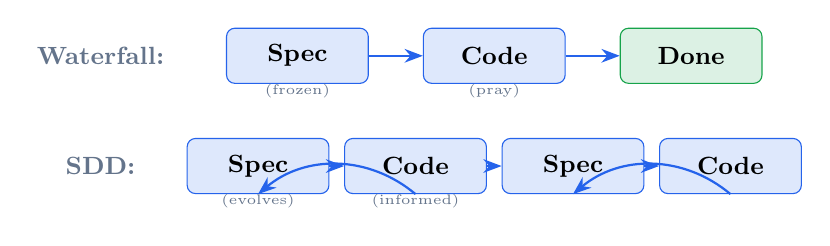
\begin{tikzpicture}[
    box/.style={rectangle, rounded corners=3pt, fill=openblue!15,
                draw=openblue, minimum width=1.8cm, minimum height=0.7cm,
                font=\small\bfseries},
    arr/.style={-{Stealth}, thick, color=openblue},
    label/.style={font=\small\bfseries, color=opengray}
  ]
    %% Waterfall
    \node[label] at (0, 2.2) {Waterfall:};
    \node[box] (ws) at (2.5, 2.2) {Spec};
    \node[box] (wc) at (5.0, 2.2) {Code};
    \node[box, fill=opengreen!15, draw=opengreen] (wd) at (7.5, 2.2) {Done};
    \node[font=\tiny\color{opengray}] at (2.5, 1.75) {(frozen)};
    \node[font=\tiny\color{opengray}] at (5.0, 1.75) {(pray)};
    \draw[arr] (ws) -- (wc);
    \draw[arr] (wc) -- (wd);

    %% SDD
    \node[label] at (0, 0.8) {SDD:};
    \node[box] (ss1) at (2.0, 0.8) {Spec};
    \node[box] (sc1) at (4.0, 0.8) {Code};
    \node[box] (ss2) at (6.0, 0.8) {Spec};
    \node[box] (sc2) at (8.0, 0.8) {Code};
    \node[font=\tiny\color{opengray}] at (2.0, 0.35) {(evolves)};
    \node[font=\tiny\color{opengray}] at (4.0, 0.35) {(informed)};
    \draw[arr] (ss1) -- (sc1);
    \draw[arr] (sc1) -- (ss2);
    \draw[arr] (ss2) -- (sc2);
    \draw[arr, bend right=40] (sc1.south) to (ss1.south);
    \draw[arr, bend right=40] (sc2.south) to (ss2.south);
  \end{tikzpicture}
  \vspace{0.5em}

  Specs and code evolve together through \textbf{feedback loops}.
\end{frame}

\begin{frame}{SDD vs TDD vs BDD}
  \vspace{0.3em}
  \begin{tabularx}{\textwidth}{l X X c}
    \toprule
    \textbf{Approach} & \textbf{Spec Source} & \textbf{Written When} & \textbf{AI-Native?} \\
    \midrule
    No specs    & Chat history     & Never              & \color{openred}Poor \\
    TDD         & Test cases       & Before code        & \color{opengray}Partial \\
    BDD         & User stories     & Before tests       & \color{opengray}Partial \\
    \textbf{SDD} & \textbf{Formal specs} & \textbf{Before everything} & \color{opengreen}\textbf{Yes} \\
    \bottomrule
  \end{tabularx}
  \vspace{1em}
  SDD is the first approach built \textbf{for} the AI era.
\end{frame}

\begin{frame}{Why Write Things Down?}
  \vspace{2em}
  \begin{center}
    \large\textit{"If you're thinking without writing,\\
    you only think you're thinking."}\\[1.2em]
    \normalsize\color{opengray}— Leslie Lamport,\\ \textit{Specifying Systems}, 2002
  \end{center}
\end{frame}

%% ══════════════════════════════════════════════
%% SECTION 4: ENTER OPENSPEC
%% ══════════════════════════════════════════════

\begin{frame}{What is OpenSpec?}
  \vspace{1.5em}
  \begin{center}
    {\Large\textbf{OpenSpec}}\\[1em]
    \normalsize
    An AI-native framework\\
    for specification-driven development.\\[1.5em]
    \small\color{opengray}MIT licensed · TypeScript · 36+ AI tools supported
  \end{center}
\end{frame}

\begin{frame}{The Numbers}
  \vspace{0.5em}
  \begin{columns}[T]
    \begin{column}{0.33\textwidth}
      \centering
      {\fontsize{40}{48}\selectfont\textbf{\color{openblue}71K+}}\\[0.3em]
      \normalsize GitHub stars
    \end{column}
    \begin{column}{0.33\textwidth}
      \centering
      {\fontsize{40}{48}\selectfont\textbf{\color{openblue}265K+}}\\[0.3em]
      \normalsize developers/month
    \end{column}
    \begin{column}{0.33\textwidth}
      \centering
      {\fontsize{40}{48}\selectfont\textbf{\color{openblue}36+}}\\[0.3em]
      \normalsize supported AI tools
    \end{column}
  \end{columns}
\end{frame}

\begin{frame}{}
  \vspace{2.5em}
  \begin{center}
    {\Large\textit{"One new spec created}}\\[0.3em]
    {\Large\textit{every two seconds."}}\\[1.5em]
    \normalsize\color{opengray}— openspec.dev
  \end{center}
\end{frame}

\begin{frame}{The Philosophy}
  \vspace{0.5em}
  \begin{center}
    \begin{tabular}{r@{\quad}l}
      {\Large\textbf{Fluid}}      & not rigid \\[0.7em]
      {\Large\textbf{Iterative}}  & not waterfall \\[0.7em]
      {\Large\textbf{Easy}}       & not complex \\[0.7em]
      {\Large\textbf{Brownfield}} & not just greenfield \\[0.7em]
      {\Large\textbf{Scalable}}   & solo dev to enterprise \\
    \end{tabular}
  \end{center}
\end{frame}

%% ── BRIDGE SLIDES ──────────────────────────────
\begin{frame}{}
  \vspace{3em}
  \begin{center}
    {\Large Let's see it in action.}
  \end{center}
\end{frame}

\begin{frame}[fragile]{Install in 30 Seconds}
\begin{lstlisting}
npm install -g @fission-ai/openspec
cd your-project
openspec init
openspec update
\end{lstlisting}
  \vspace{0.8em}
  Done. Your AI tools are now spec-aware.
\end{frame}

\begin{frame}{The Mental Model}
  \vspace{0.3em}
  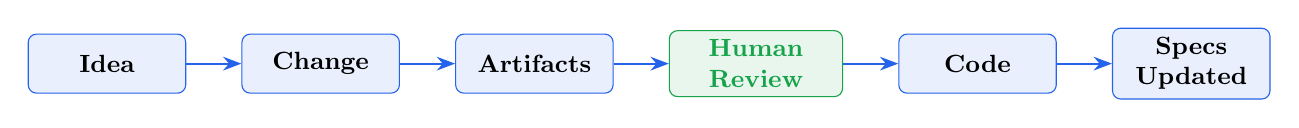
\begin{tikzpicture}[
    box/.style={rectangle, rounded corners=3pt, draw=openblue, fill=openblue!10,
                minimum width=2cm, minimum height=0.75cm, align=center,
                font=\small\bfseries},
    rev/.style={rectangle, rounded corners=3pt, draw=opengreen, fill=opengreen!10,
                minimum width=2.2cm, minimum height=0.75cm, align=center,
                font=\small\bfseries, text=opengreen},
    arr/.style={-{Stealth}, thick, color=openblue},
    lbl/.style={font=\tiny\color{opengray}, above=0.15cm}
  ]
    \node[box] (idea)  {Idea};
    \node[box, right=0.7cm of idea]  (chg)  {Change};
    \node[box, right=0.7cm of chg]   (art)  {Artifacts};
    \node[rev, right=0.7cm of art]   (rev)  {Human\\Review};
    \node[box, right=0.7cm of rev]   (code) {Code};
    \node[box, right=0.7cm of code]  (spec) {Specs\\Updated};

    \draw[arr] (idea) -- (chg);
    \draw[arr] (chg)  -- (art);
    \draw[arr] (art)  -- (rev);
    \draw[arr] (rev)  -- (code);
    \draw[arr] (code) -- (spec);
  \end{tikzpicture}
  \vspace{0.8em}

  Every change is \textbf{planned before built},\\
  \textbf{reviewed before implemented},\\
  \textbf{archived after done}.
\end{frame}

%% ══════════════════════════════════════════════
%% SECTION 5: CORE CONCEPTS
%% ══════════════════════════════════════════════

\begin{frame}[fragile]{Specs}
  \textbf{Specs = Requirements + Scenarios}\\[0.5em]
  Plain Markdown files defining what the system SHALL do.
  \vspace{0.3em}
\begin{lstlisting}
## Requirements
- SHALL support light and dark themes
- SHALL persist user preference

## Scenarios
- WHEN user toggles theme
  THEN UI updates immediately
- WHEN user reopens app
  THEN last theme is restored
\end{lstlisting}
\end{frame}

\begin{frame}[fragile]{Changes}
  \textbf{A Change = A Self-Contained Proposal}\\[0.8em]
\begin{lstlisting}
openspec/changes/add-dark-mode/
  |-  proposal.md
  |-  design.md
  |-  tasks.md
  `-  specs/
\end{lstlisting}
  \vspace{0.8em}
  Everything about one change lives in one folder.
\end{frame}

\begin{frame}{Proposals}
  \textbf{\texttt{proposal.md} — The Why and What}\\[1em]
  \begin{itemize}\setlength\itemsep{0.5em}
    \item What problem are we solving?
    \item What is \textbf{in scope}?
    \item What is explicitly \textbf{OUT of scope}?
  \end{itemize}
  \vspace{1em}
  The proposal is the contract between human and AI.
\end{frame}

\begin{frame}{Design}
  \textbf{\texttt{design.md} — The How}\\[1em]
  \begin{itemize}\setlength\itemsep{0.5em}
    \item Technical approach
    \item Architecture decisions
    \item Trade-offs considered
  \end{itemize}
  \vspace{1em}
  Written by AI, \textbf{reviewed by human}.
\end{frame}

\begin{frame}[fragile]{Tasks}
  \textbf{\texttt{tasks.md} — The Checklist}\\[0.5em]
\begin{lstlisting}
- [ ] Add CSS custom properties for colors
- [ ] Create ThemeToggle component
- [ ] Add localStorage persistence
- [ ] Update components to use theme variables
- [ ] Add tests for theme switching
\end{lstlisting}
  \vspace{0.5em}
  Discrete, implementable units of work.
\end{frame}

\begin{frame}{The Golden Rule}
  \vspace{2em}
  \begin{center}
    {\Large\textbf{"AI creates artifacts.}}\\[0.5em]
    {\Large\textbf{Human reviews.}}\\[0.5em]
    {\Large\textbf{AI implements."}}
  \end{center}
\end{frame}

%% ══════════════════════════════════════════════
%% SECTION 6: THE WORKFLOW
%% ══════════════════════════════════════════════

\begin{frame}{The Four Phases}
  \vspace{0.5em}
  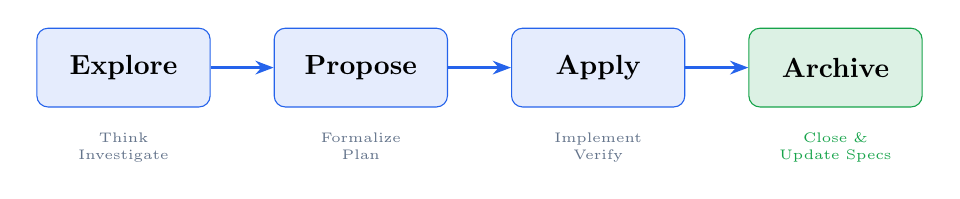
\begin{tikzpicture}[
    box/.style={rectangle, rounded corners=4pt, draw=openblue,
                fill=openblue!12, minimum width=2.2cm, minimum height=1.0cm,
                text centered, font=\bfseries},
    sub/.style={font=\tiny\color{opengray}, text width=2.2cm, align=center},
    arr/.style={-{Stealth}, thick, color=openblue}
  ]
    \node[box] (e) {Explore};
    \node[box, right=0.8cm of e] (p) {Propose};
    \node[box, right=0.8cm of p] (a) {Apply};
    \node[box, right=0.8cm of a, fill=opengreen!15, draw=opengreen] (ar) {Archive};

    \draw[arr] (e) -- (p);
    \draw[arr] (p) -- (a);
    \draw[arr] (a) -- (ar);

    \node[sub, below=0.2cm of e] {Think\\Investigate};
    \node[sub, below=0.2cm of p] {Formalize\\Plan};
    \node[sub, below=0.2cm of a] {Implement\\Verify};
    \node[sub, below=0.2cm of ar, text=opengreen] {Close \&\\Update Specs};
  \end{tikzpicture}
  \vspace{0.8em}

  A full cycle from idea to done.
\end{frame}

\begin{frame}[fragile]{Explore}
  \Large\texttt{/opsx:explore}\\[1em]
  \normalsize
  \begin{itemize}\setlength\itemsep{0.5em}
    \item Investigate the codebase
    \item Ask questions, think freely
    \item No commitments, no files written
    \item Pure discovery
  \end{itemize}
  \vspace{1em}
  \textit{"Thinking time, not task time."}
\end{frame}

\begin{frame}[fragile]{Propose}
  \Large\texttt{/opsx:propose add-dark-mode}\\[1em]
  \normalsize
  \begin{itemize}\setlength\itemsep{0.5em}
    \item Creates change folder with all artifacts
    \item AI drafts proposal, design, specs, tasks
    \item Human reviews and approves each artifact
  \end{itemize}
  \vspace{1em}
  \textbf{Nothing is built until YOU say so.}
\end{frame}

\begin{frame}[fragile]{Apply}
  \Large\texttt{/opsx:apply}\\[1em]
  \normalsize
  \begin{itemize}\setlength\itemsep{0.5em}
    \item Implements tasks one by one
    \item Each task verified before moving to next
    \item AI follows the design, not its imagination
  \end{itemize}
  \vspace{1em}
  The spec is the guardrail.
\end{frame}

\begin{frame}[fragile]{Archive}
  \Large\texttt{/opsx:archive}\\[1em]
  \normalsize
  \begin{itemize}\setlength\itemsep{0.5em}
    \item Change is completed and archived
    \item Main specs updated with new requirements
    \item History preserved for future reference
  \end{itemize}
  \vspace{1em}
  The loop closes. Specs are the living record.
\end{frame}

%% ══════════════════════════════════════════════
%% SECTION 7: REAL EXAMPLE
%% ══════════════════════════════════════════════

\begin{frame}{Example: "Add Dark Mode"}
  \vspace{1em}
  \begin{center}
    \Large We want to add \textbf{dark mode} to our web app.\\[1.5em]
    \normalsize
    \textbf{Without specs:}\\
    "Hey AI, add dark mode" → unpredictable result\\[1em]
    \textbf{With OpenSpec:}\\
    structured, reviewed, implemented step by step
  \end{center}
\end{frame}

\begin{frame}[fragile]{The Proposal}
  \textbf{\texttt{proposal.md}}\\[0.3em]
\begin{lstlisting}
## Summary
Add dark mode with user preference persistence.

## In Scope
- Theme toggle component
- CSS custom properties for theming
- localStorage persistence

## Out of Scope
- System preference detection (future)
- Per-page theme overrides
\end{lstlisting}
  \small\color{opengray}Clear boundaries. AI knows what \textbf{NOT} to do.
\end{frame}

\begin{frame}[fragile]{The Design}
  \textbf{\texttt{design.md}}\\[0.3em]
\begin{lstlisting}
## Approach
Use CSS custom properties on :root.
Toggle class on <html> element.

## Decision: CSS Variables vs CSS-in-JS
CSS variables chosen for:
- Zero runtime cost
- Works with existing stylesheets
- No library dependency
\end{lstlisting}
  \small\color{opengray}Decisions documented, not buried in comments.
\end{frame}

\begin{frame}[fragile]{The Tasks}
  \textbf{\texttt{tasks.md}}\\[0.3em]
\begin{lstlisting}
- [ ] Define color tokens in :root
      and [data-theme="dark"]
- [ ] Create ThemeToggle component
- [ ] Wire toggle to localStorage
- [ ] Migrate hardcoded colors
- [ ] Add unit tests for ThemeToggle
\end{lstlisting}
  \small\color{opengray}Each task is independently implementable and verifiable.
\end{frame}

\begin{frame}[fragile]{After Archive}
  \vspace{0.5em}
  \begin{columns}[T]
    \begin{column}{0.48\textwidth}
      \textbf{Before:}
\begin{lstlisting}
specs/
  (no theming spec)
\end{lstlisting}
    \end{column}
    \begin{column}{0.48\textwidth}
      \textbf{After:}
\begin{lstlisting}
specs/theming/spec.md
  - SHALL support light
    and dark themes
  - SHALL persist pref
    in localStorage
\end{lstlisting}
    \end{column}
  \end{columns}
  \vspace{0.8em}
  The spec becomes the \textbf{permanent record}.\\
  Next time anyone touches theming — the spec is there.
\end{frame}

%% ══════════════════════════════════════════════
%% SECTION 8: ADVANCED FEATURES
%% ══════════════════════════════════════════════

\begin{frame}{Stores: Cross-Repo Planning}
  \vspace{0.3em}
  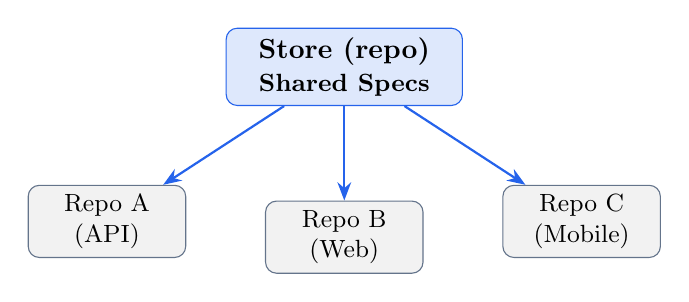
\begin{tikzpicture}[
    store/.style={rectangle, rounded corners, draw=openblue, fill=openblue!15,
                  minimum width=3cm, minimum height=0.9cm, font=\bfseries,
                  align=center, text centered},
    repo/.style={rectangle, rounded corners, draw=opengray, fill=gray!10,
                 minimum width=2cm, minimum height=0.7cm, font=\small,
                 align=center, text centered},
    arr/.style={-{Stealth}, thick, color=openblue}
  ]
    \node[store] (s) {Store (repo)\\\small Shared Specs};
    \node[repo, below left=1cm and 0.5cm of s] (a) {Repo A\\(API)};
    \node[repo, below=1.2cm of s] (b) {Repo B\\(Web)};
    \node[repo, below right=1cm and 0.5cm of s] (c) {Repo C\\(Mobile)};
    \draw[arr] (s) -- (a);
    \draw[arr] (s) -- (b);
    \draw[arr] (s) -- (c);
  \end{tikzpicture}
  \vspace{0.5em}

  Platform teams publish specs.\\
  Product teams consume them.
\end{frame}

\begin{frame}{36+ Supported Tools}
  \vspace{0.5em}
  \begin{center}
    \large Works with your \textbf{existing} setup.\\[1em]
    \normalsize
    Claude Code \textbullet{} GitHub Copilot \textbullet{} Cursor \textbullet{} Amazon Q\\[0.5em]
    Codeium \textbullet{} Windsurf \textbullet{} Aider \textbullet{} Continue \textbullet{} Zed\\[0.5em]
    JetBrains AI \textbullet{} VS Code \textbullet{} and more...\\[1em]
    \textbf{No vendor lock-in. MIT licensed.}
  \end{center}
\end{frame}

\begin{frame}[fragile]{Brownfield Ready}
  \vspace{0.5em}
  \large You don't need to start from scratch.\\[1em]
\begin{lstlisting}
cd your-existing-project
openspec init
\end{lstlisting}
  \vspace{0.8em}
  \normalsize
  Two commands. Your existing code stays untouched.\\[0.5em]
  Specs describe what you build \textbf{next}, not what already exists.
\end{frame}

\begin{frame}[fragile]{Keeping AI in Sync}
  \Large\texttt{openspec update}\\[1em]
  \normalsize
  \begin{itemize}\setlength\itemsep{0.5em}
    \item Refreshes AI instruction files in your project
    \item Run after updating OpenSpec or changing config
    \item Ensures every AI tool reads the latest specs and rules
  \end{itemize}
  \vspace{1em}
  \textit{"Your AI assistants are only as good\\
  as their instructions."}
\end{frame}

%% ══════════════════════════════════════════════
%% SECTION 9: COMPARISONS
%% ══════════════════════════════════════════════

\begin{frame}{vs GitHub Spec Kit}
  \vspace{0.5em}
  \begin{tabularx}{\textwidth}{l X X}
    \toprule
    & \textbf{OpenSpec} & \textbf{Spec Kit} \\
    \midrule
    Weight      & Lightweight        & Heavyweight \\
    Workflow    & Iterative          & Rigid phase gates \\
    Setup       & \texttt{npm i -g openspec} & Python environment \\
    Flexibility & Any AI tool        & GitHub ecosystem \\
    \bottomrule
  \end{tabularx}
  \vspace{1em}
  \color{opengray}\textit{"Thorough but heavyweight."} — OpenSpec comparison
\end{frame}

\begin{frame}{vs AWS Kiro}
  \vspace{0.5em}
  \begin{tabularx}{\textwidth}{l X X}
    \toprule
    & \textbf{OpenSpec} & \textbf{Kiro} \\
    \midrule
    IDE      & Any (36+ tools)     & Kiro IDE only \\
    Models   & Any LLM             & Claude only \\
    Approach & Spec-first          & IDE-integrated \\
    Lock-in  & None (MIT)          & AWS ecosystem \\
    \bottomrule
  \end{tabularx}
  \vspace{1em}
  \color{opengray}\textit{"Powerful but locked into their IDE."} — OpenSpec comparison
\end{frame}

\begin{frame}{vs No Framework}
  \vspace{0.5em}
  \begin{tabularx}{\textwidth}{l X X}
    \toprule
    & \textbf{OpenSpec} & \textbf{No Framework} \\
    \midrule
    Requirements & Versioned Markdown  & Chat history \\
    Persistence  & Git-tracked specs   & Gone when chat closes \\
    Review       & Human approves      & Hope for the best \\
    Consistency  & Enforced by specs   & Random \\
    \bottomrule
  \end{tabularx}
  \vspace{1em}
  \Large\textbf{"Hope is not a strategy."}
\end{frame}

%% ══════════════════════════════════════════════
%% SECTION 10: CONTROVERSIES
%% ══════════════════════════════════════════════

\begin{frame}{Fair Criticism}
  \vspace{1.5em}
  \begin{center}
    \Large Not everyone is convinced.\\[1em]
    \normalsize Let's be honest about the objections.
  \end{center}
\end{frame}

\begin{frame}{Controversy \#1}
  \vspace{0.5em}
  \begin{center}
    \large\textit{"This is just waterfall in disguise."}
  \end{center}
  \vspace{0.8em}
  \begin{columns}[T]
    \begin{column}{0.48\textwidth}
      \textbf{\color{openred}The critique}\\[0.4em]
      \small Agile killed BDUF in 2001.\\
      Writing specs first = Big Design Up Front.\\
      We're going backwards.
    \end{column}
    \begin{column}{0.48\textwidth}
      \textbf{\color{opengreen}The reality}\\[0.4em]
      \small OpenSpec specs \textit{evolve}.\\
      Waterfall specs were frozen.\\
      Iterative $\neq$ specless.
    \end{column}
  \end{columns}
\end{frame}

\begin{frame}{Controversy \#2}
  \vspace{0.5em}
  \begin{center}
    \large\textit{"AI doesn't actually read specs."}
  \end{center}
  \vspace{0.8em}
  \begin{columns}[T]
    \begin{column}{0.48\textwidth}
      \textbf{\color{openred}The critique}\\[0.4em]
      \small LLMs are probabilistic.\\
      Context windows overflow.\\
      AI "agrees" then ignores constraints.
    \end{column}
    \begin{column}{0.48\textwidth}
      \textbf{\color{opengreen}The reality}\\[0.4em]
      \small OpenSpec is designed around this.\\
      Structured context $>$ chat soup.\\
      Human review catches drift.
    \end{column}
  \end{columns}
\end{frame}

\begin{frame}{Controversy \#3}
  \vspace{0.5em}
  \begin{center}
    \large\textit{"Garbage in, garbage out."}
  \end{center}
  \vspace{0.8em}
  \begin{columns}[T]
    \begin{column}{0.48\textwidth}
      \textbf{\color{openred}The critique}\\[0.4em]
      \small A wrong spec perfectly implemented\\
      is still wrong.\\
      Who validates the specs?
    \end{column}
    \begin{column}{0.48\textwidth}
      \textbf{\color{opengreen}The reality}\\[0.4em]
      \small This is actually a \textbf{feature}.\\
      Bad assumptions become\\
      explicit and traceable.
    \end{column}
  \end{columns}
\end{frame}

\begin{frame}{The Honest Answer}
  \vspace{0.5em}
  \large OpenSpec is not a silver bullet.\\[1em]
  \normalsize
  \begin{itemize}\setlength\itemsep{0.5em}
    \item It adds overhead — especially for tiny projects
    \item AI models still hallucinate, specs or not
    \item Bad specs produce bad software, faster
  \end{itemize}
  \vspace{0.8em}
  \textbf{But:} the alternative is unstructured prompting\\
  at scale. That's worse.

\end{frame}

%% ══════════════════════════════════════════════
%% SECTION 11: CLOSING
%% ══════════════════════════════════════════════

\begin{frame}{Why This Matters}
  \vspace{0.5em}
  \large AI without specs is chaos on a longer horizon.\\[1.5em]
  \normalsize
  One feature? Fine.\\[0.3em]
  Ten features? Cracks appear.\\[0.3em]
  A full product? \textbf{Unmanageable without specs.}
\end{frame}

\begin{frame}{Specs $\neq$ Waterfall}
  \vspace{0.5em}
  \large\textbf{Specification-Driven $\neq$ Waterfall}\\[1em]
  \normalsize
  \begin{itemize}\setlength\itemsep{0.5em}
    \item Specs are lightweight Markdown
    \item They evolve iteratively
    \item They are AI-native — written and consumed by AI
    \item Human stays in control
  \end{itemize}
\end{frame}

\begin{frame}{}
  \vspace{3em}
  \begin{center}
    {\Large\textbf{"Agree before you build."}}
  \end{center}
\end{frame}

\begin{frame}{Thank You}
  \vspace{0.5em}
  \begin{center}
    \Large\textbf{Questions?}\\[1.5em]
    \normalsize
    \begin{tabular}{rl}
      GitHub: & \texttt{\href{https://github.com/Fission-AI/openspec}{\color{openblue}github.com/Fission-AI/openspec}} \\[0.5em]
      Website: & \texttt{\href{https://openspec.dev}{\color{openblue}openspec.dev}} \\[0.5em]
      Install: & \texttt{npm install -g @fission-ai/openspec} \\[0.5em]
      Me: & \texttt{\href{https://github.com/sukhoy94}{\color{openblue}github.com/sukhoy94}} \\
    \end{tabular}
  \end{center}
\end{frame}

\end{document}
